\documentclass{article}
\usepackage[utf8]{inputenc}
\usepackage{graphicx}
\usepackage{wrapfig}
\usepackage{array}
\usepackage{siunitx}
\usepackage{xcolor}
\usepackage{multicol}
\usepackage{amssymb}
\usepackage{hyperref}
\setlength{\columnseprule}{1pt}

\title{Study of Operational Amplifier \\ Lab Report 6 \\ ELP100}
\author{Yash Agarwal \\ 2021EE10638 \\ Group 29}
\date{May 31, 2022}

\begin{document}
\pagecolor{yellow!15}
\maketitle
\vspace{15px}
\tableofcontents
\newcolumntype{V}{>{\centering\arraybackslash} m{.4\linewidth} }
\newpage
\section{Voltage Follower}
\subsection{Aim}
To setup the voltage follower and measure the output characteristics.
\subsection{Apparatus}
\begin{enumerate}
\item Breadboard and Jumpers
\item Multimeter and Resistors
\item LM741 IC
\item Digital Storage Oscilloscope (DSO1052B)
\item Function Generator (0 – 3 MHz)
\end{enumerate}

\subsection{Theory}
\begin{wrapfigure}{R}{0.35\textwidth}
\fcolorbox{black}{white}{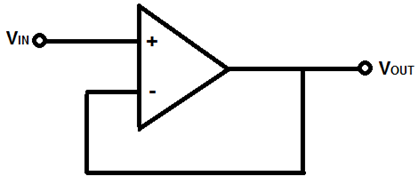
\includegraphics[width=0.35\textwidth]{Picture1.png}}
\end{wrapfigure}
A voltage follower (also called a unity-gain amplifier, a buffer amplifier, and an isolation amplifier) is a op-amp circuit which has a voltage gain of 1. This means that the op amp does not provide any amplification to the signal. The reason it is called a voltage follower is because the output voltage directly follows the input voltage, meaning the output voltage is the same as the input voltage. An op amp circuit is a circuit with a very high input impedance. This high input impedance is the reason voltage followers are used. When a circuit has a very high input impedance, very little current is drawn from the circuit. If you know ohm's law, you know that current, I=V/R. Thus, the greater the resistance, the less current is drawn from a power source. Hence, voltage follower draws very less current due to which they do not load down the power source. There is too much use of voltage follower because an op amp has a very high input impedance, the majority of voltage will fall across it, (since it's so high impedance). So it's very valuable when used in a voltage divider circuit because strategically doing so can allow a designer to supply sufficient voltage to a load.

\begin{center}
    \textbf{$V_{in}=V_{out}$}
\end{center}


\newpage

\subsection{Breadboard Setup}
\vspace{5px}
\begin{center}
\fcolorbox{black}{white}{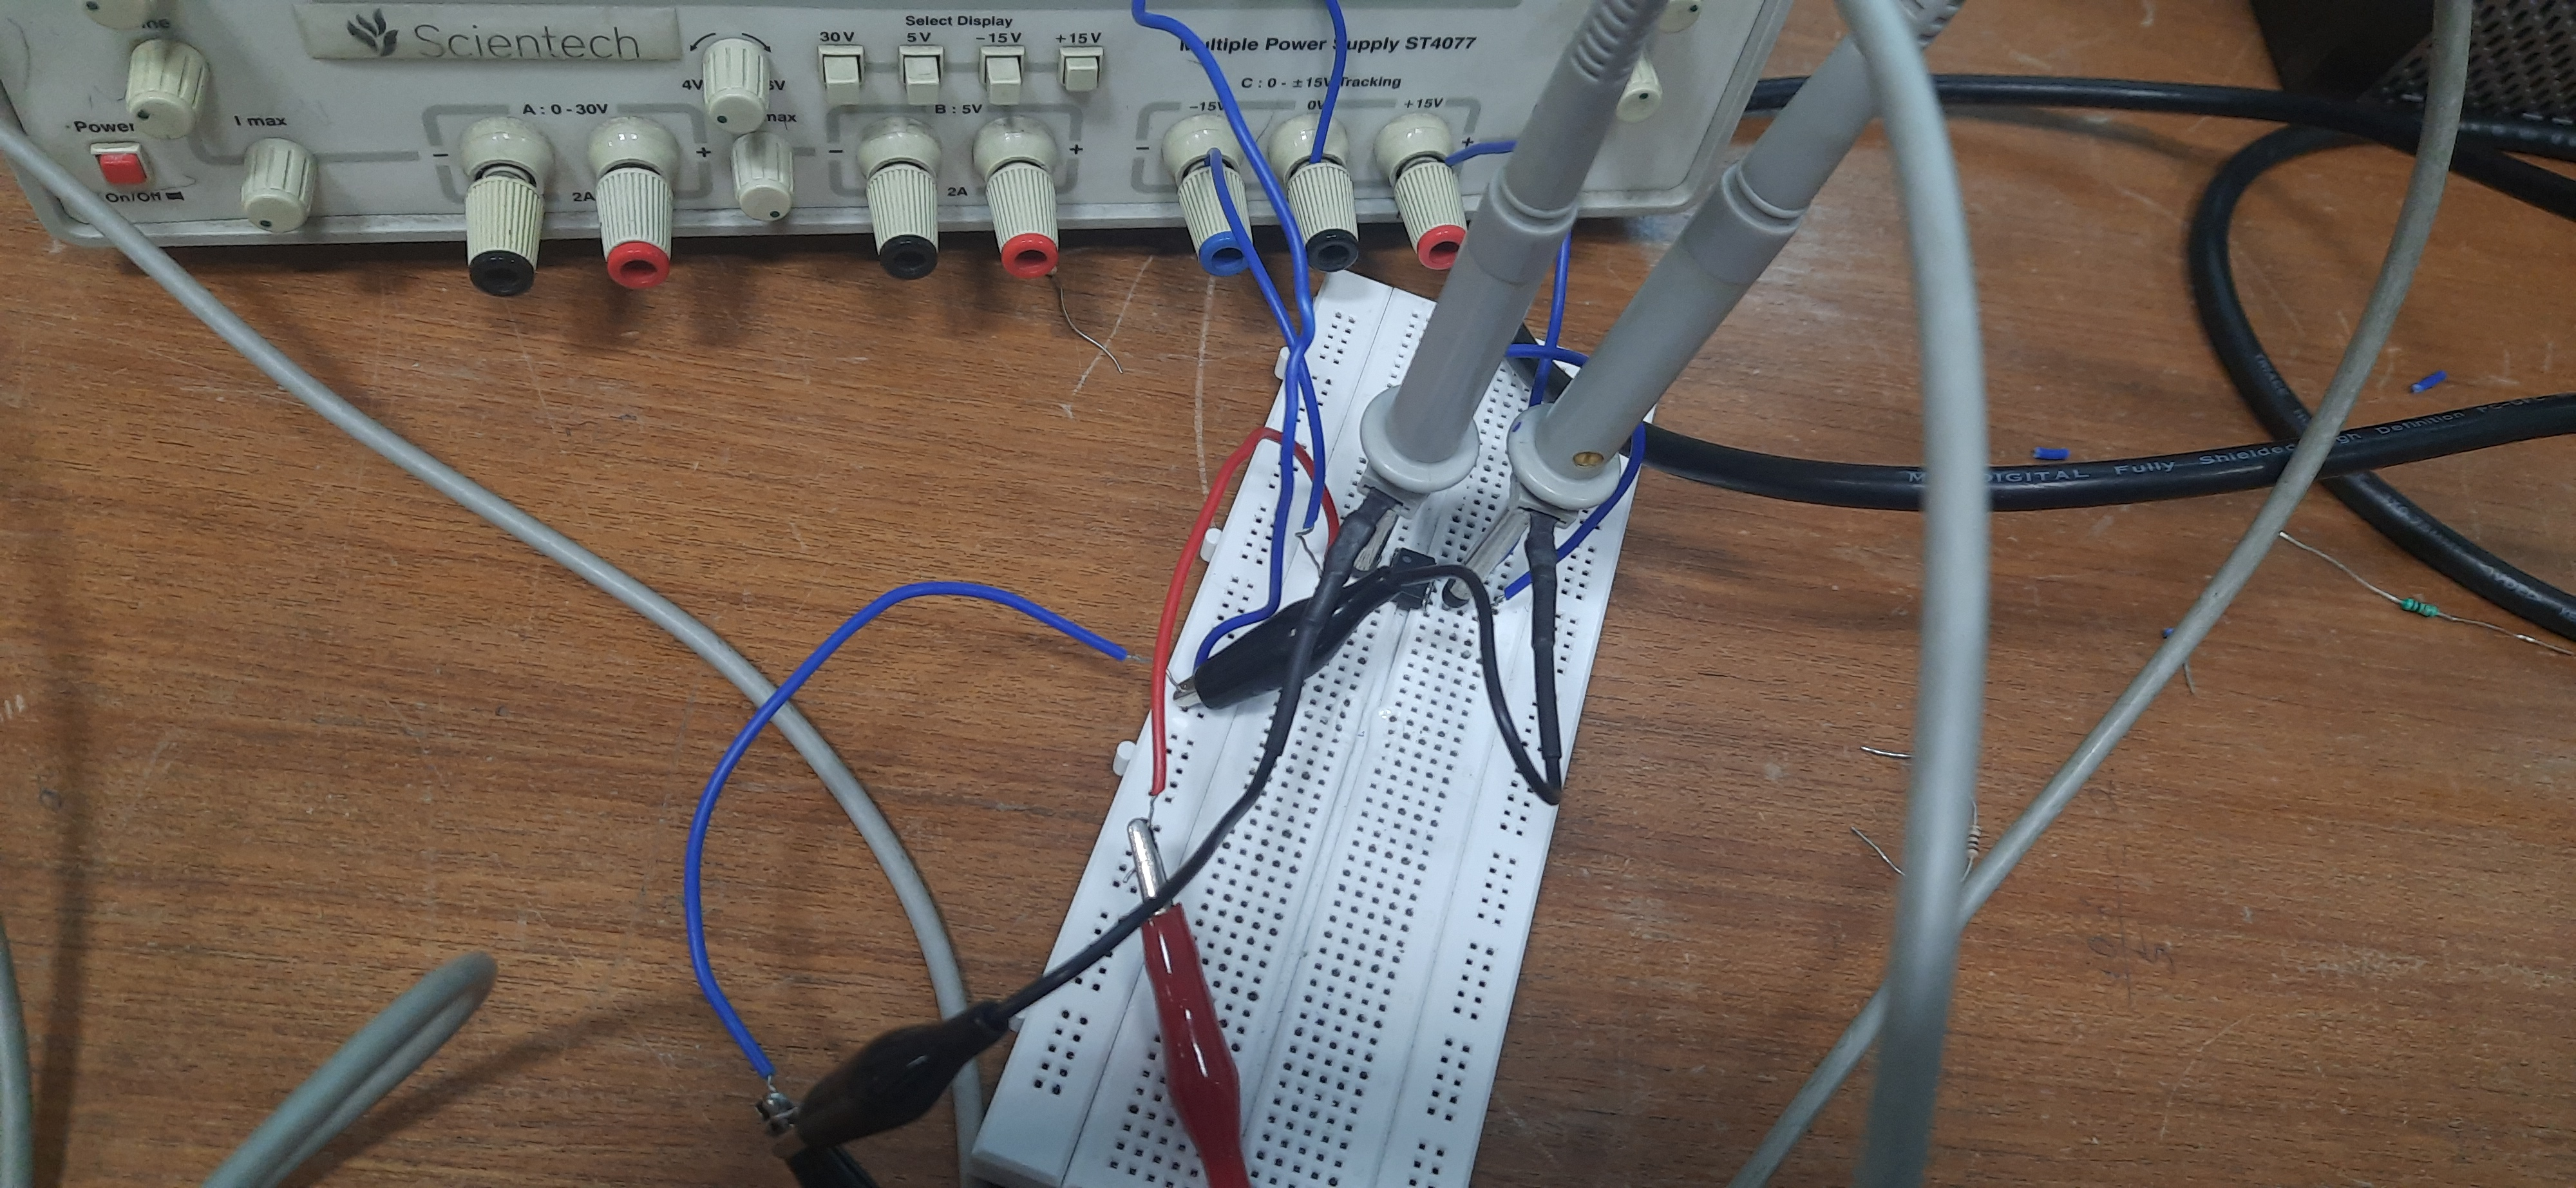
\includegraphics[width=0.9\columnwidth, height=150px]{20220517_160615.jpg}} \\ \vspace{5px}
Circuit\\

\vspace{5px}
\fcolorbox{black}{white}{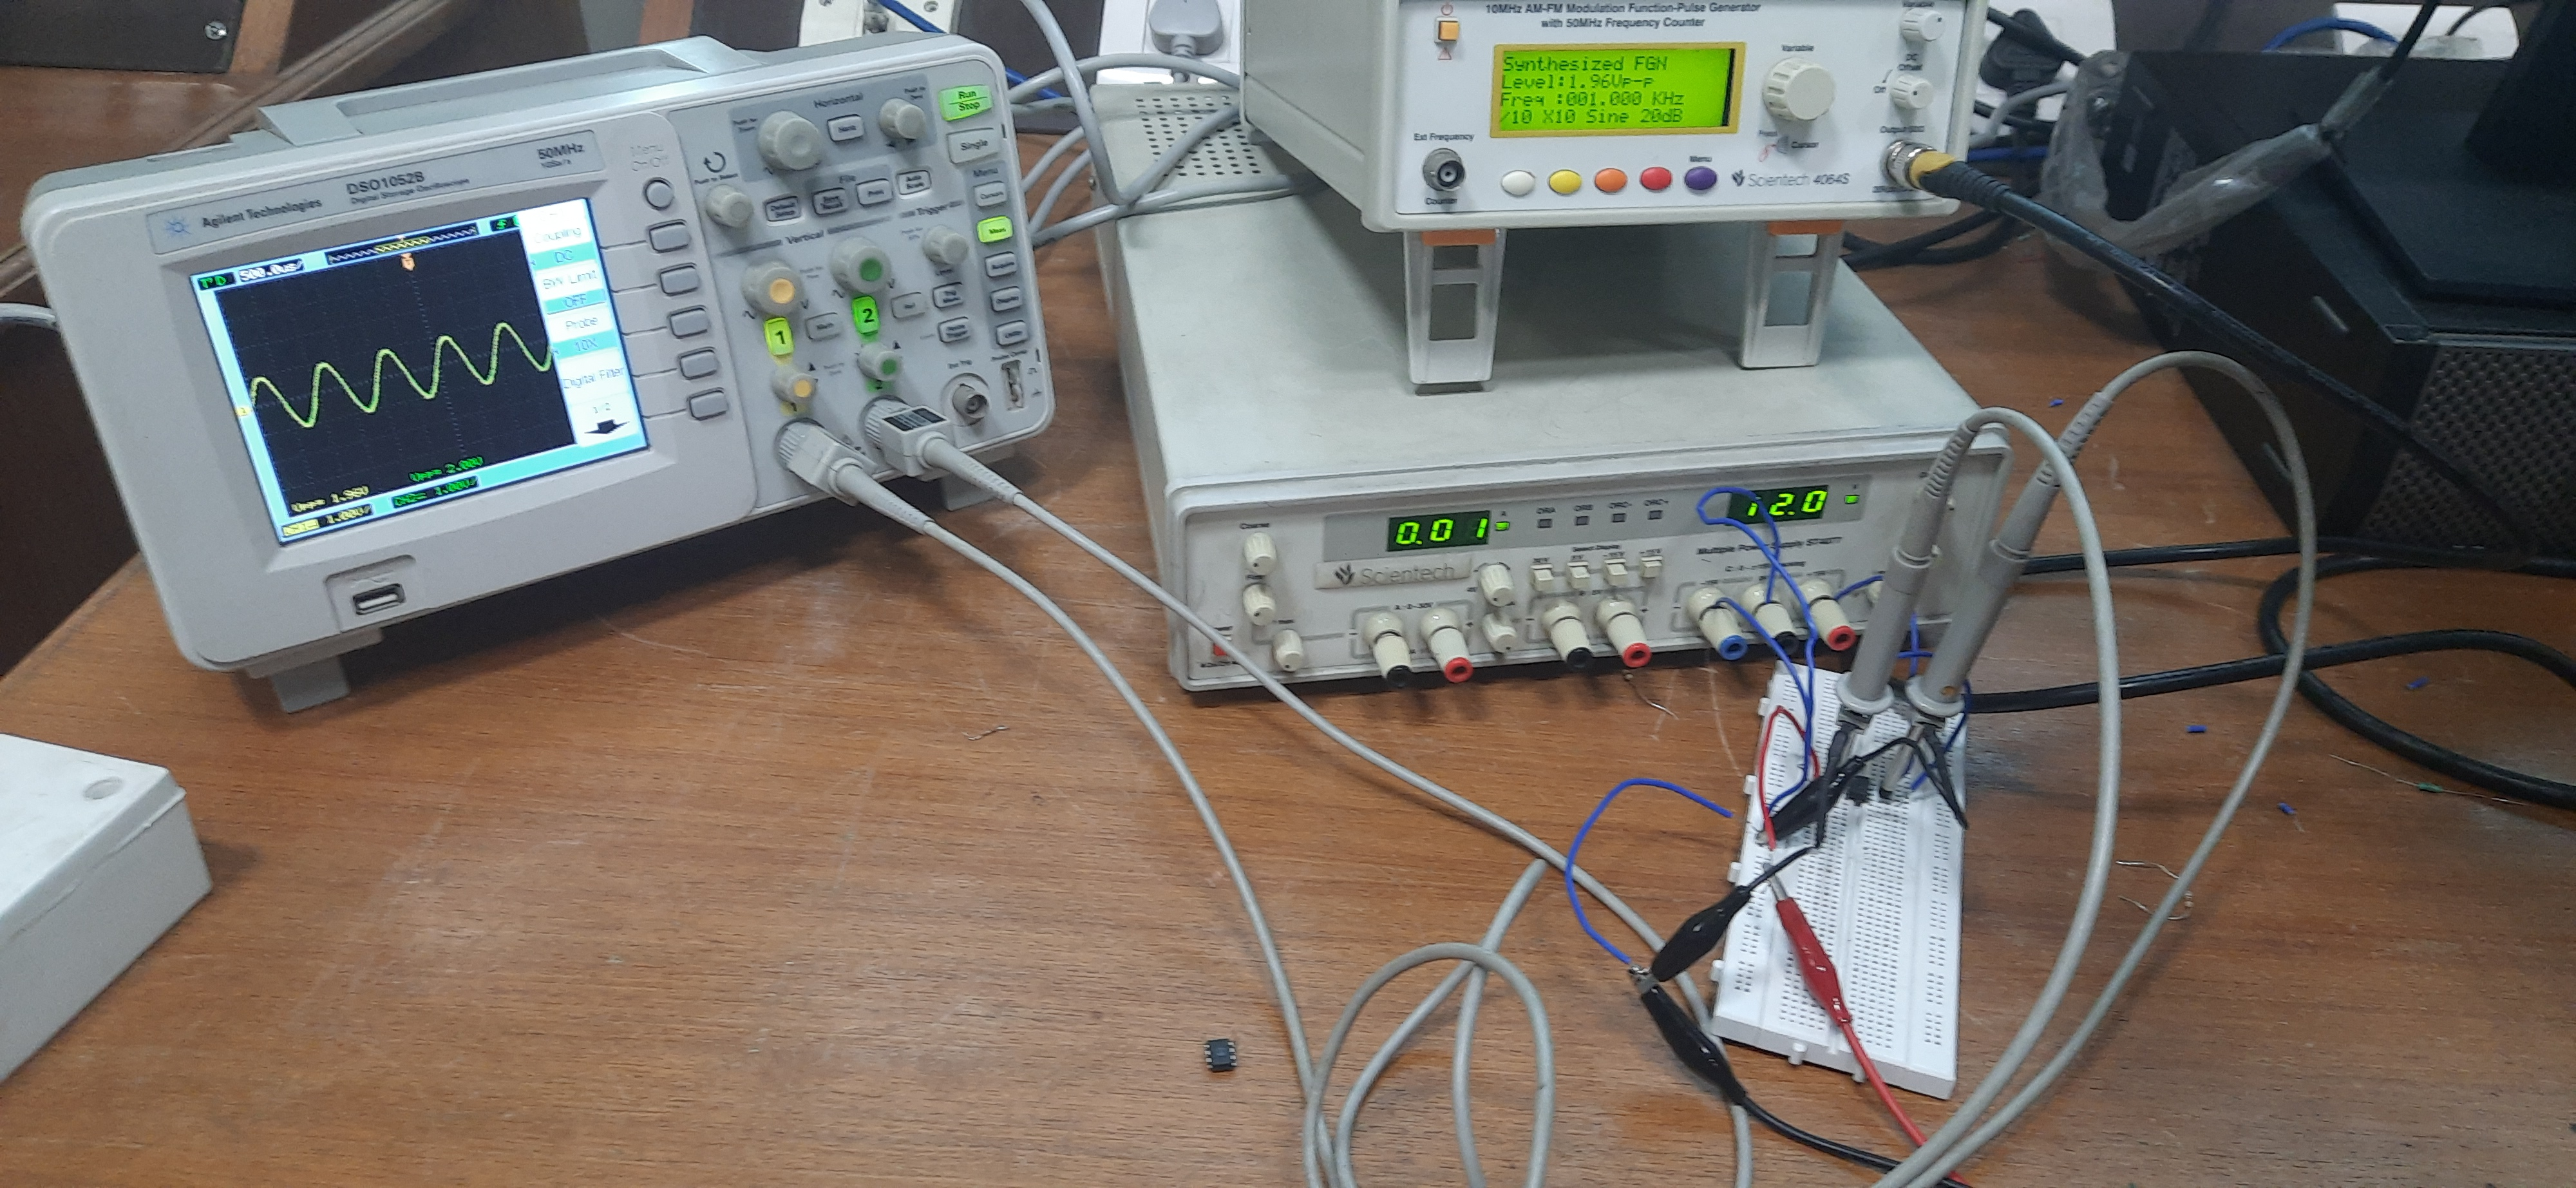
\includegraphics[width=0.9\columnwidth, height=150px]{20220517_160619.jpg}} \\ \vspace{5px}
Circuit with DSO
\end{center}

\subsection{Images of DSO}
\vspace{5px}
\begin{multicols}{2}
\begin{center}
\fcolorbox{black}{white}{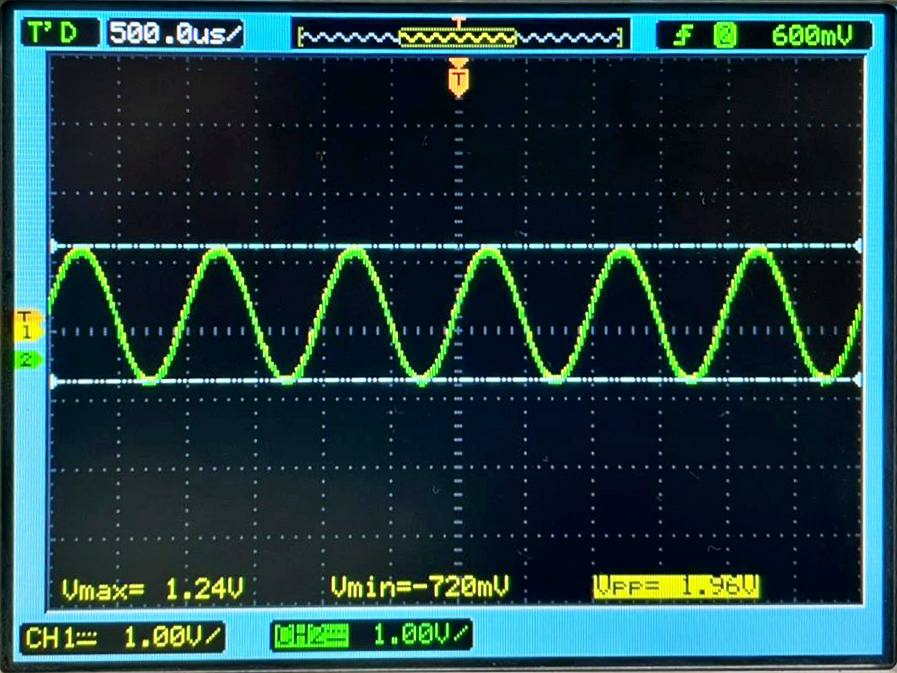
\includegraphics[width=0.9\columnwidth, height=110px]{WhatsApp Image 2022-05-31 at 5.34.40 PM.jpeg}} \\ \vspace{5px}
Voltage Follower\\

\columnbreak

\fcolorbox{black}{white}{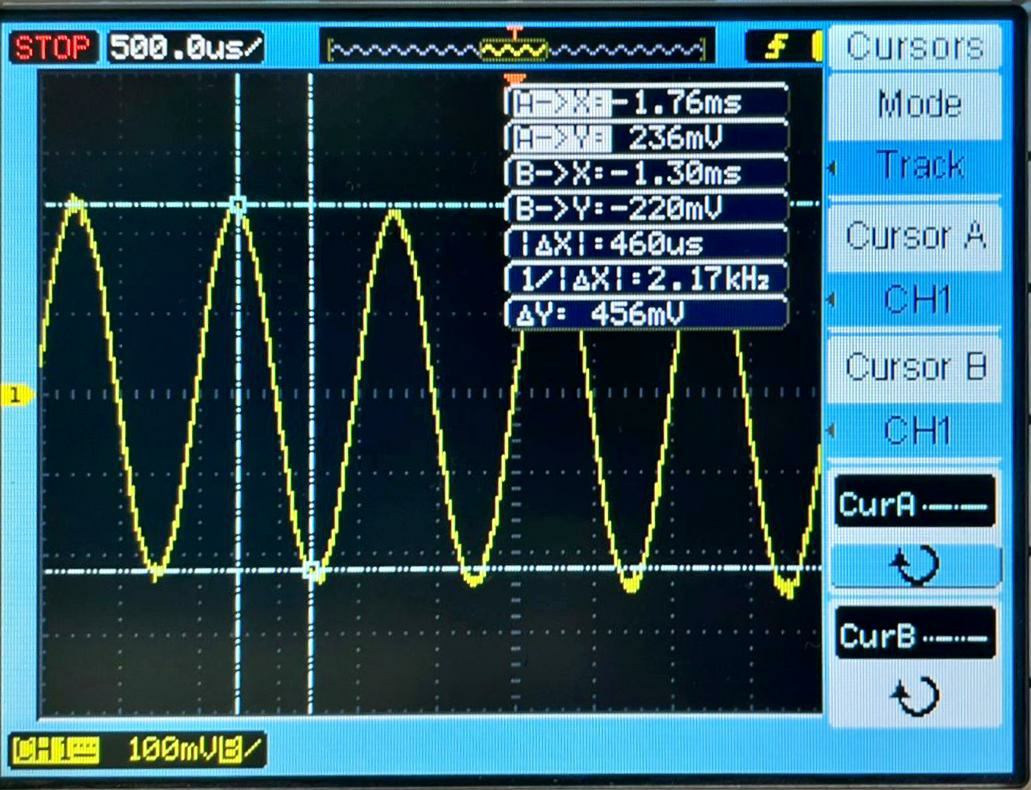
\includegraphics[width=0.9\columnwidth, height=110px]{WhatsApp Image 2022-05-31 at 5.34.40 PM (1).jpeg}} \\ \vspace{5px}
Voltage with 100$\Omega$ Resistor 
\end{center}
\end{multicols}

\subsection{Observation}
\vspace{5px}
\begin{center}
\begin{tabular}{| c | c | c |} 
 \hline
    \ & \ & \ \\
    $V_{Input}$ & $V_{Output}$ & $V_{Output}$ with Resistor \\ [1em]
    \hline
    \ & \ & \ \\
    2.00V & 1.96V & 456mV \\
    \ & \ & \ \\
 \hline
\end{tabular}
\end{center}

\subsection{Conclusion}
Thus, we see that the Output Voltage drops to 456mV when we connect the 100$\Omega$ resistor in parallel across the generator and the DSO input. However, when we connect the input signal to the DSO via the Voltage Follower, the op-amp maintains the input signal voltage to give an approximately same output.

\newpage
\section{Inverting Amplifier}
\subsection{Aim}
To measure the output current characteristics of an inverting amplifier.
\subsection{Apparatus}
\begin{enumerate}
\item Breadboard and Jumpers
\item Multimeter and Resistors
\item LM741 IC
\item Digital Storage Oscilloscope (DSO1052B)
\item Function Generator (0 – 3 MHz) and External Voltage
\end{enumerate}

\subsection{Theory}
\begin{wrapfigure}{R}{0.35\textwidth}
\fcolorbox{black}{white}{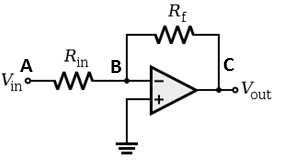
\includegraphics[width=0.35\textwidth]{Picture2.png}}
\end{wrapfigure}
The gain equation can be derived in the following manner, \\ V-$\approx$V+=0V (Virtual Ground Method). \\

\noindent
By KCL, $\frac{V_{in}}{R_{in}}$+$\frac{V_{out}}{R_{f}}$=0 \\

\begin{center}
    \textbf{$V_{out}=-V{in}\times\frac{R_{f}}{R_{in}}$}
\end{center}

\subsection{Breadboard Setup}
\vspace{5px}
\begin{center}
\fcolorbox{black}{white}{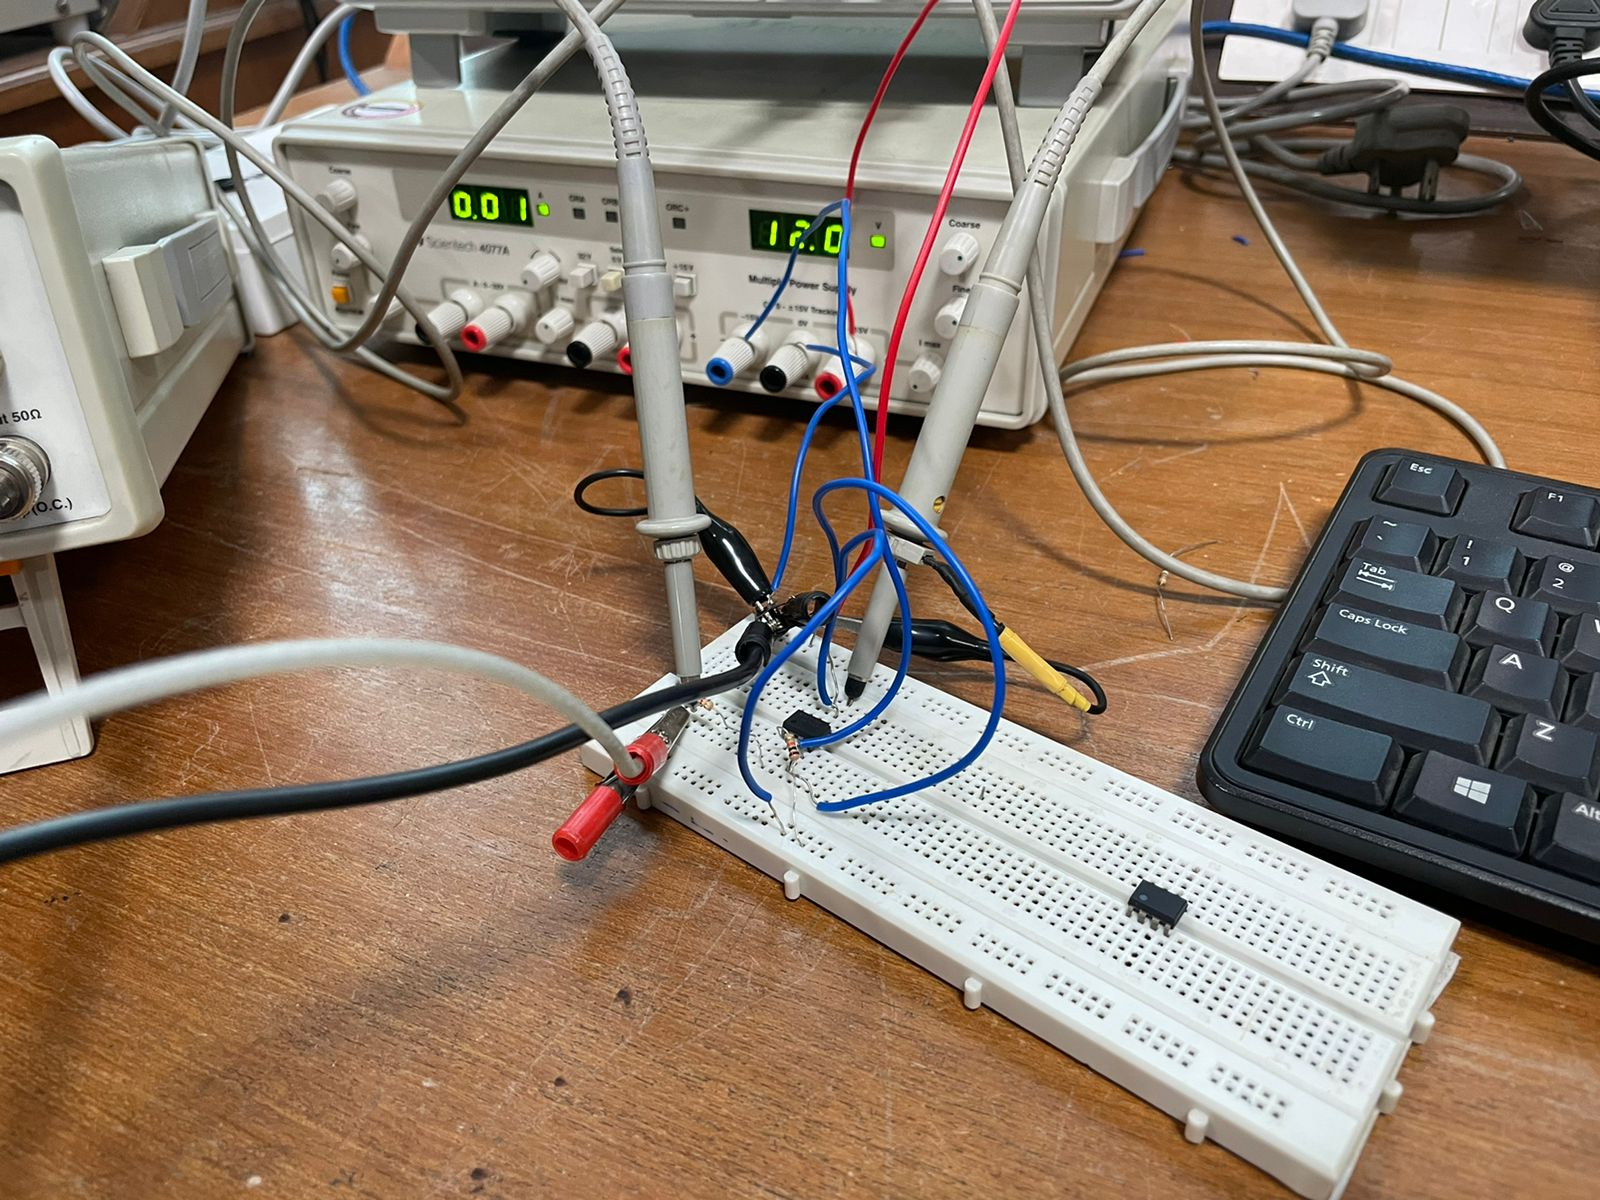
\includegraphics[width=0.9\columnwidth, height=150px]{WhatsApp Image 2022-05-30 at 5.49.31 PM.jpeg}} \\ \vspace{5px}
Circuit with $R_{in}=1k\Omega$ and $R_{f}=10k\Omega$\\
\end{center}

\newpage
\subsection{Images of DSO}
\begin{multicols}{2}
\begin{center}
\fcolorbox{black}{white}{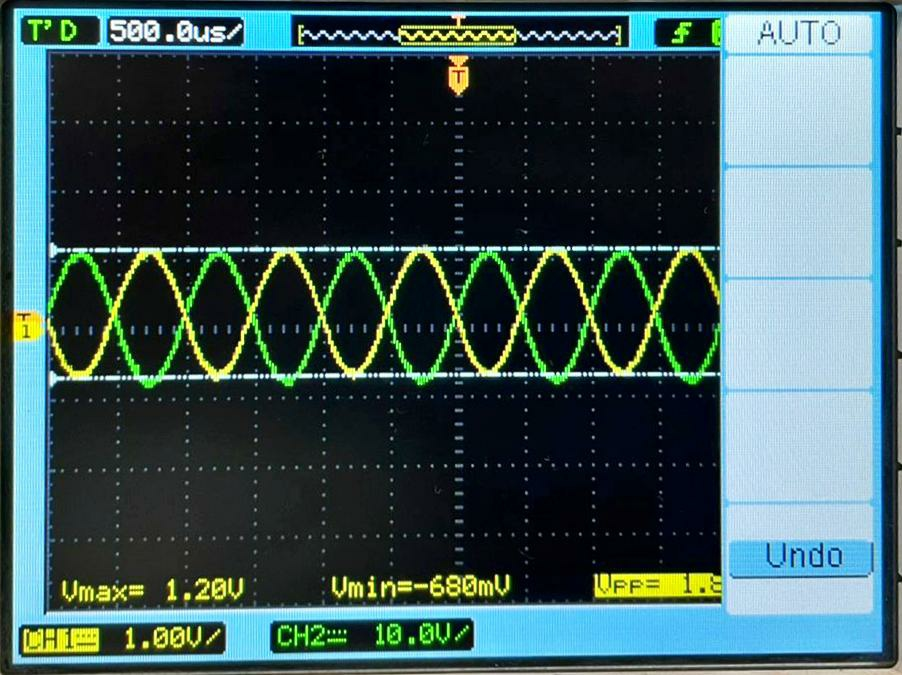
\includegraphics[width=0.9\columnwidth, height=110px]{WhatsApp Image 2022-05-31 at 9.20.08 PM (3).jpeg}} \\ \vspace{5px} 
F=1kHz \ $R_f=10k\Omega$ \\

\columnbreak

\fcolorbox{black}{white}{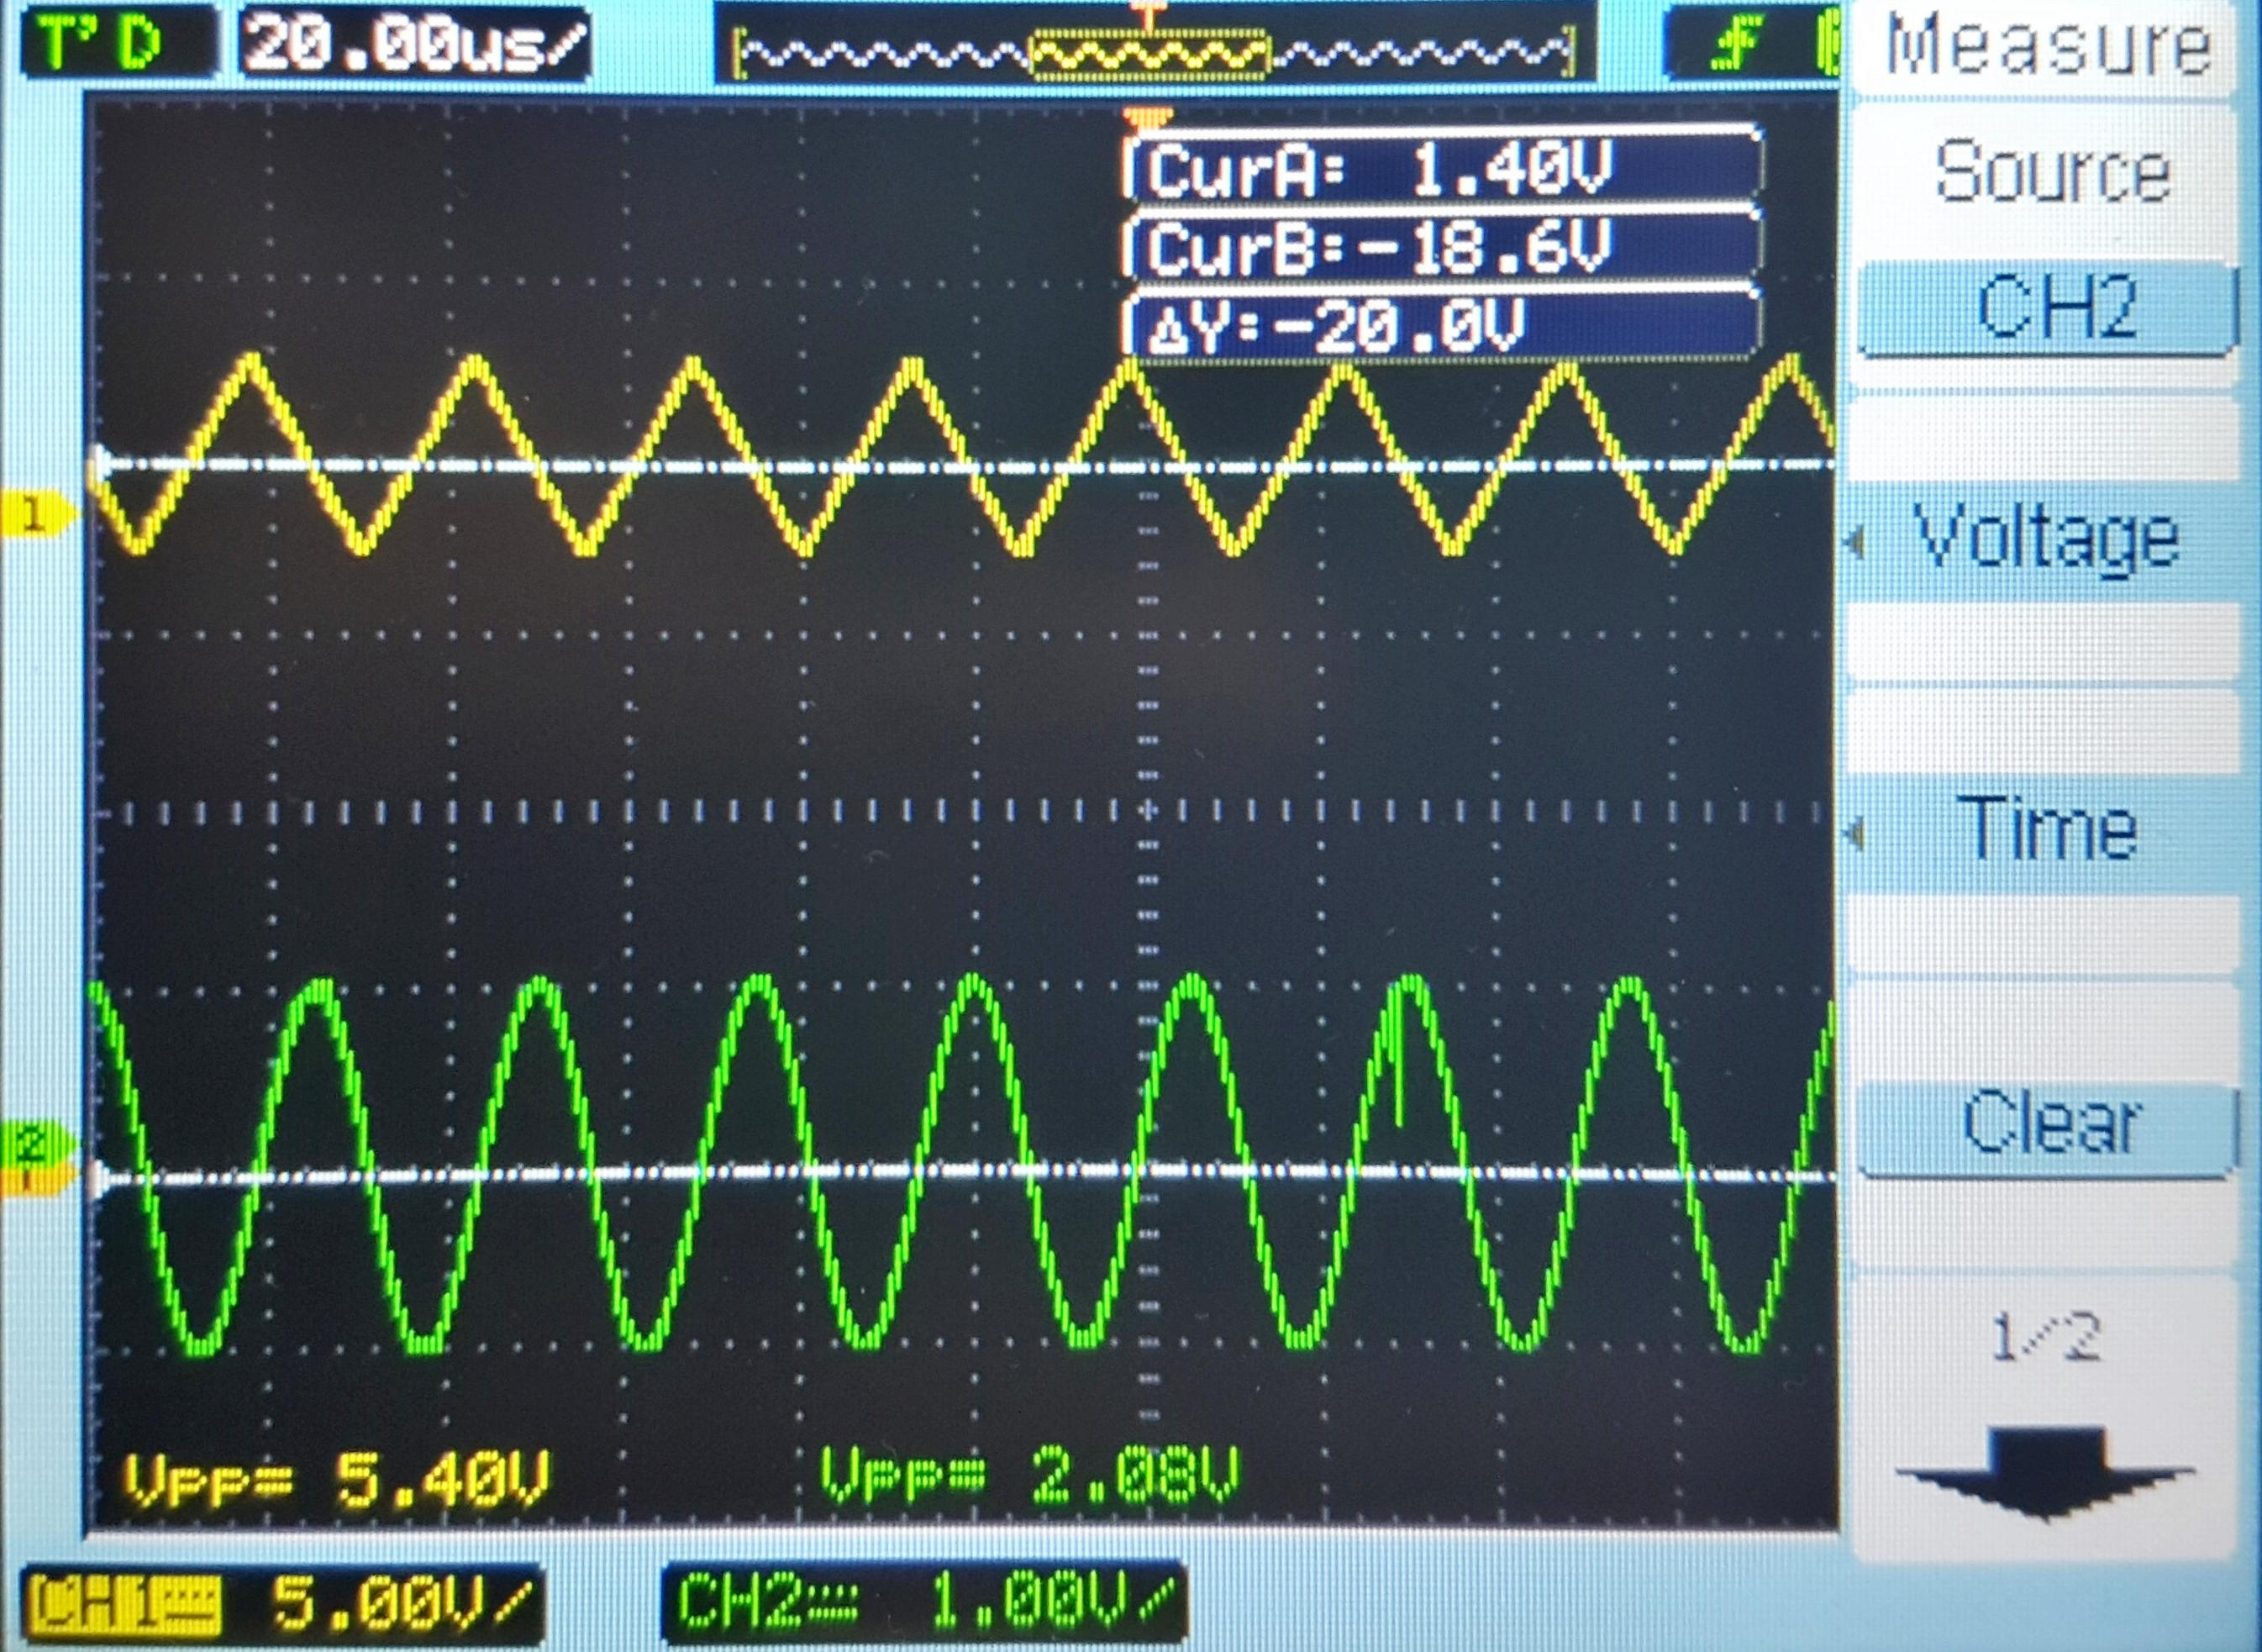
\includegraphics[width=0.9\columnwidth, height=110px]{WhatsApp Image 2022-05-31 at 9.20.08 PM (1).jpeg}} \\ \vspace{5px}
F=40kHz \ $R_f=10k\Omega$
\end{center}
\end{multicols}
\begin{multicols}{2}
\begin{center}
\fcolorbox{black}{white}{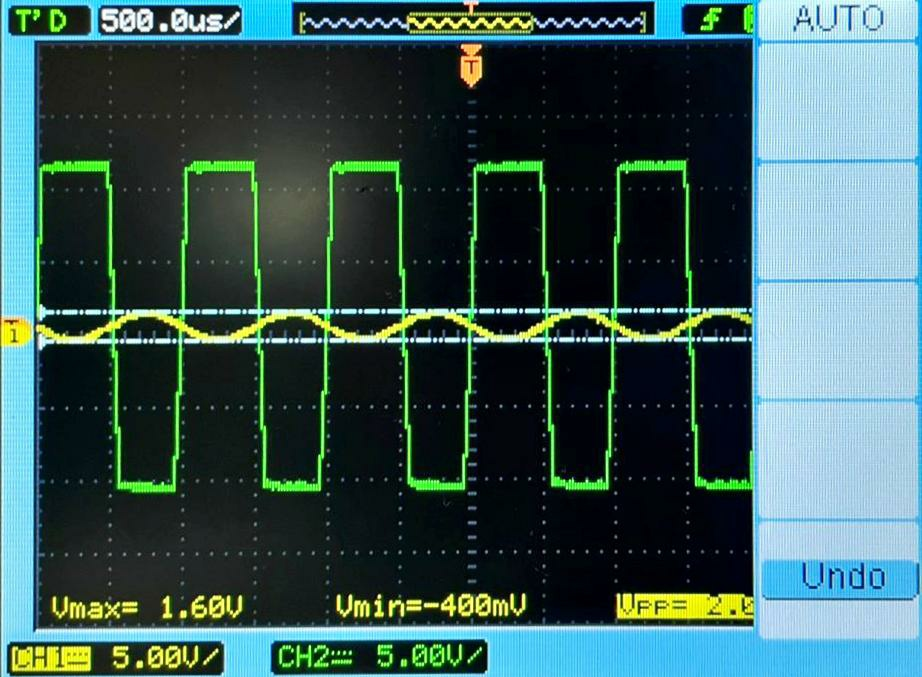
\includegraphics[width=0.9\columnwidth, height=110px]{WhatsApp Image 2022-05-31 at 9.20.08 PM (2).jpeg}} \\ \vspace{5px}
F=1kHz \ $R_f=47k\Omega$ \\

\columnbreak

\fcolorbox{black}{white}{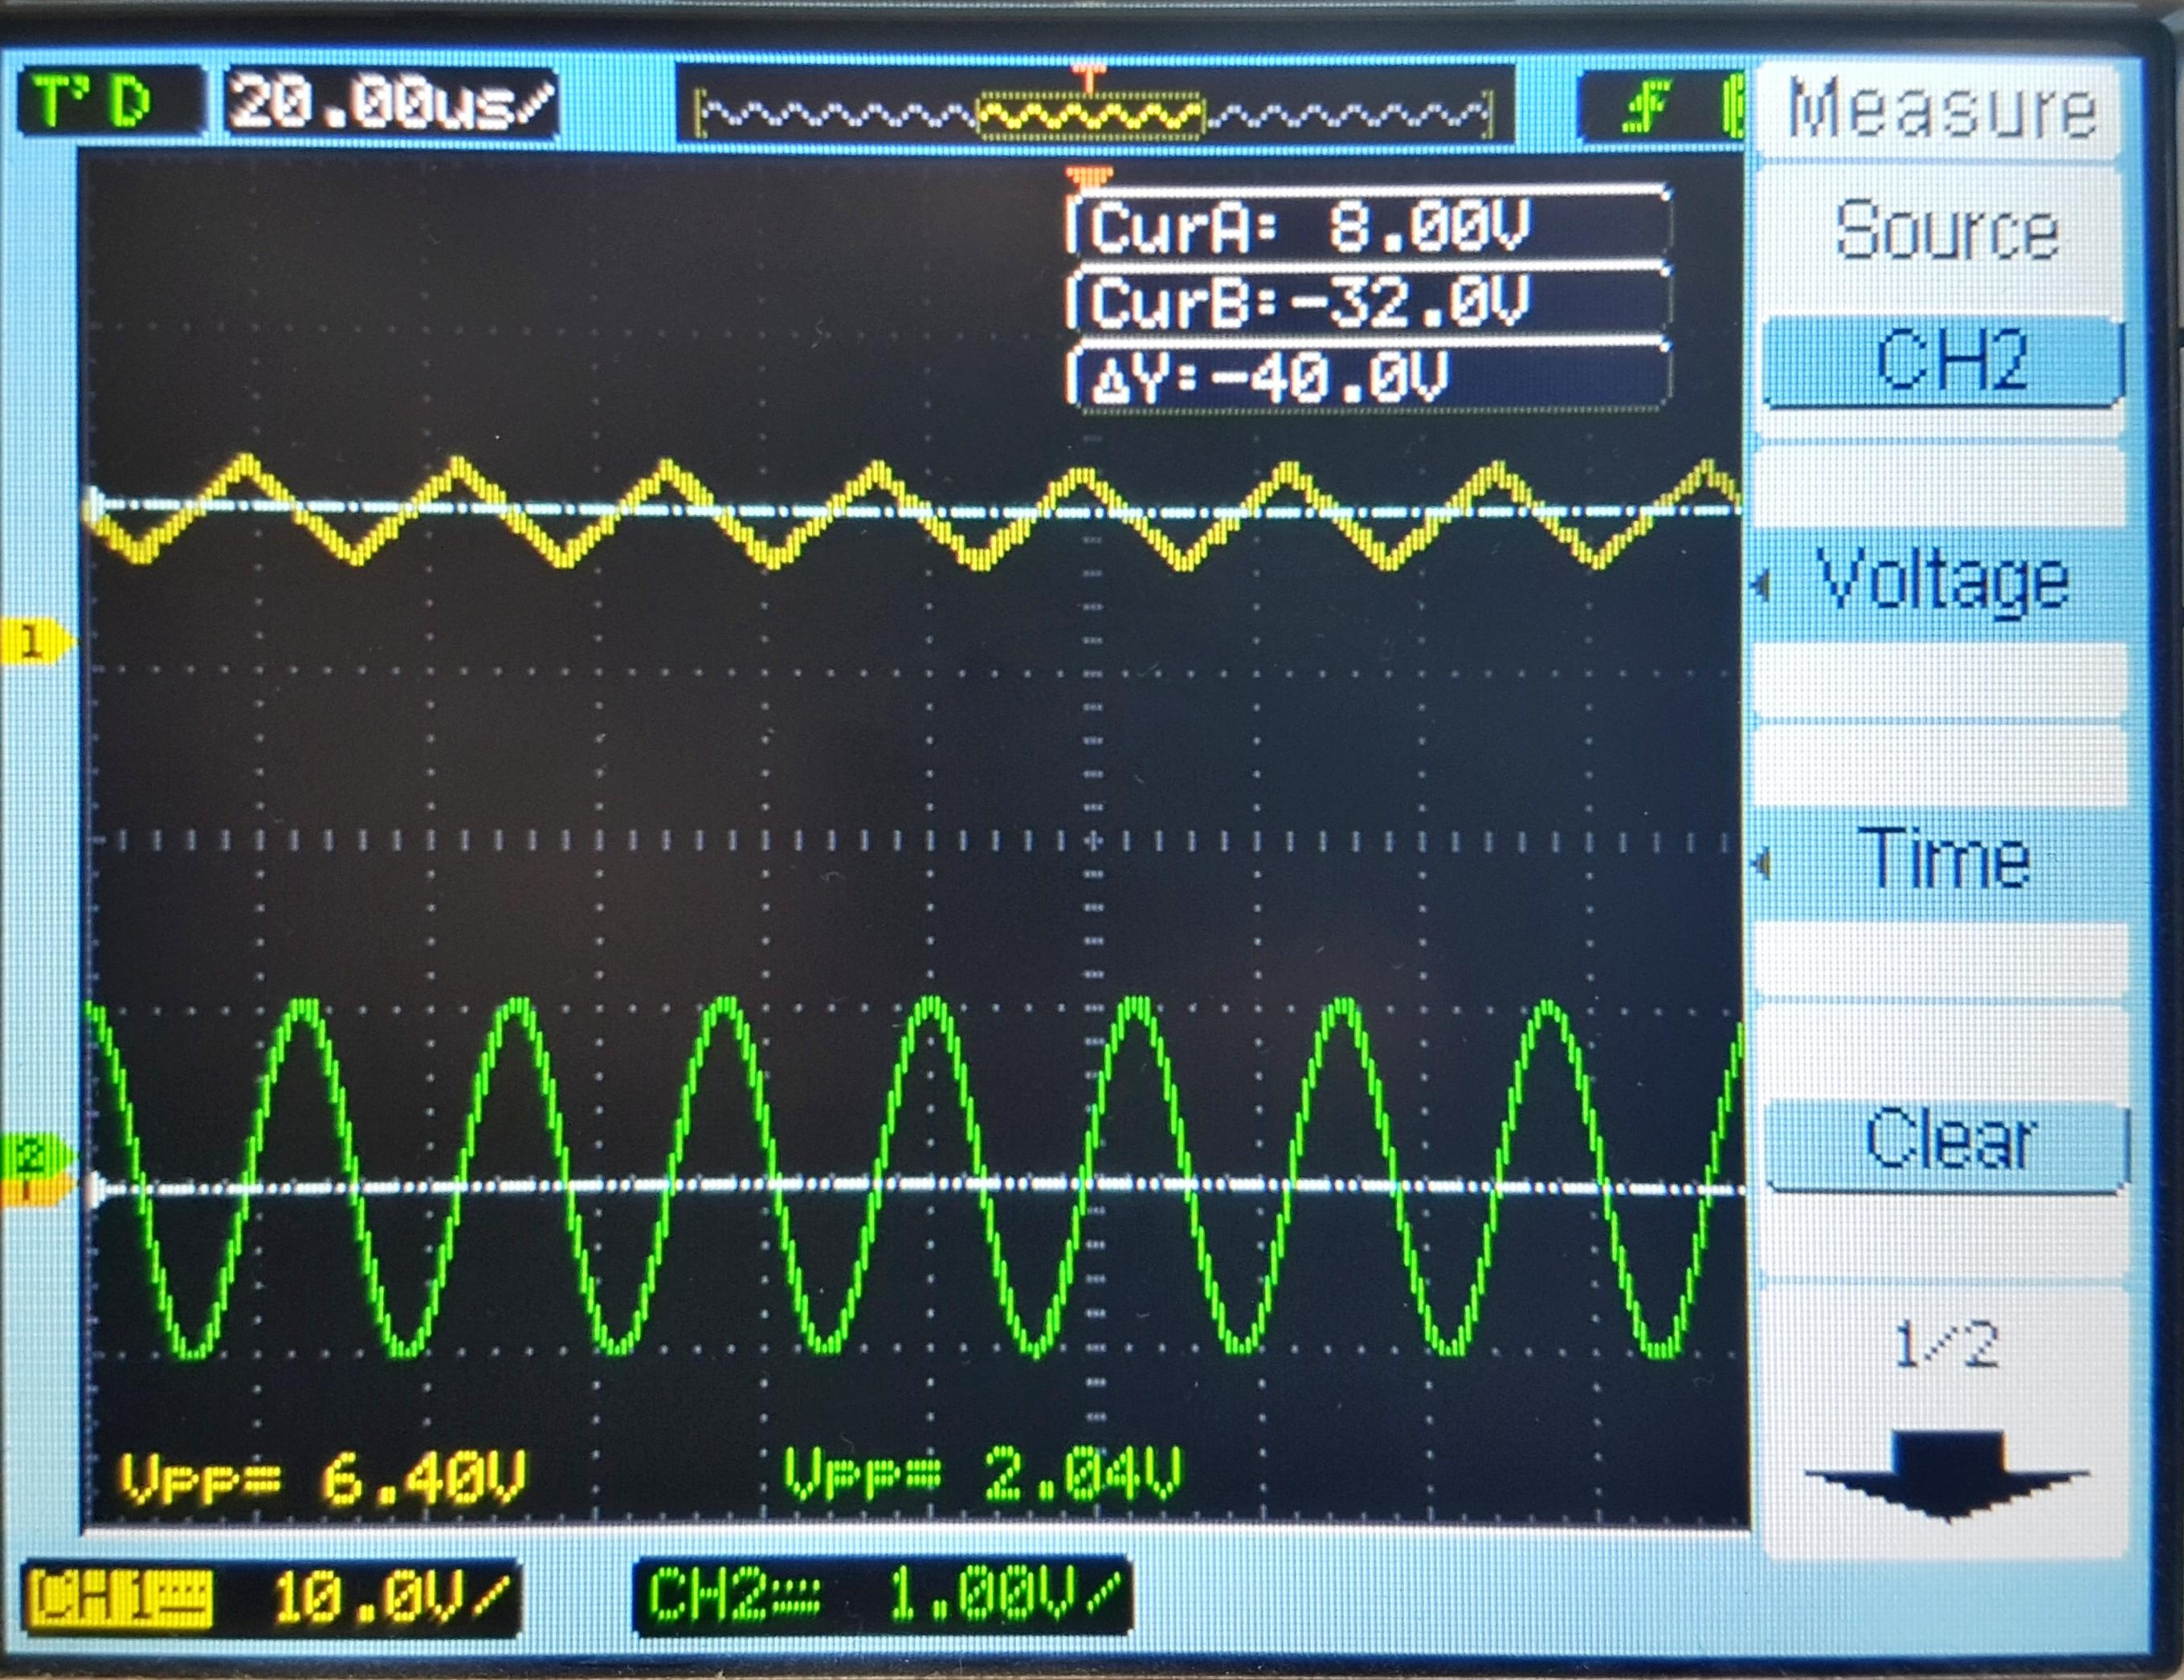
\includegraphics[width=0.9\columnwidth, height=110px]{WhatsApp Image 2022-05-31 at 9.20.08 PM.jpeg}} \\ \vspace{5px}
F=40kHz \ $R_f=47k\Omega$
\end{center}
\end{multicols}

\subsection{Observation}
\begin{center}
\begin{tabular}{| c | c | c |} 
 \hline
    \ & \ & \ \\
    Frequency and Resistance & $Input_{PP}$ & $Output_{PP}$ \\ [1em]
    \hline
    \ & \ & \ \\
    F=1kHz \ $R_f=10k\Omega$  & 2V & -20V \\
    F=40kHz \ $R_f=10k\Omega$  & 2V & -5.4V \\
    F=1kHz \ $R_f=47k\Omega$  & 2V & -22.4V \\
    F=40kHz \ $R_f=47k\Omega$  & 2V & -5.8V \\
    \ & \ & \ \\
 \hline
\end{tabular}
\end{center}

\subsection{Conclusion}
Hence, we have determined the output signal characteristics for an input sinusoidal wave for an op-amp in an inverting configuration. We see that the value of output voltage is exactly 10 times the input voltage for $R_f$ = 10k$\Omega$, which adheres to the formula. However, in $R_f$ = 47k$\Omega$ case, the value doesn’t exceed the supplied voltage. In the higher frequency shift we see higher deviations from expected results.


\newpage
\section{Non-Inverting Amplifier}
\subsection{Aim}
To measure the output current characteristics of an inverting amplifier.
\subsection{Apparatus}
\begin{enumerate}
\item Breadboard and Jumpers
\item Multimeter and Resistors
\item LM741 IC
\item Digital Storage Oscilloscope (DSO1052B)
\item Function Generator (0 – 3 MHz) and External Voltage
\end{enumerate}

\subsection{Theory}
\begin{wrapfigure}{R}{0.35\textwidth}
\fcolorbox{black}{white}{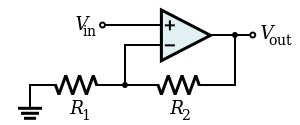
\includegraphics[width=0.35\textwidth]{Picture3.png}}
\end{wrapfigure}
The gain equation can be derived in the following manner, \\ V-$\approx$V+=$V_{in}$ (Virtual Ground Method). \\

\noindent
By KCL, $\frac{V_{in}}{R_{1}}$+$\frac{V_{in}-V_{out}}{R_{2}}$=0 \\

\begin{center}
    \textbf{$V_{out}=V{in}\times(1+\frac{R_{2}}{R_{1}})$}
\end{center}

\subsection{Breadboard Setup}
\vspace{5px}
\begin{center}
\fcolorbox{black}{white}{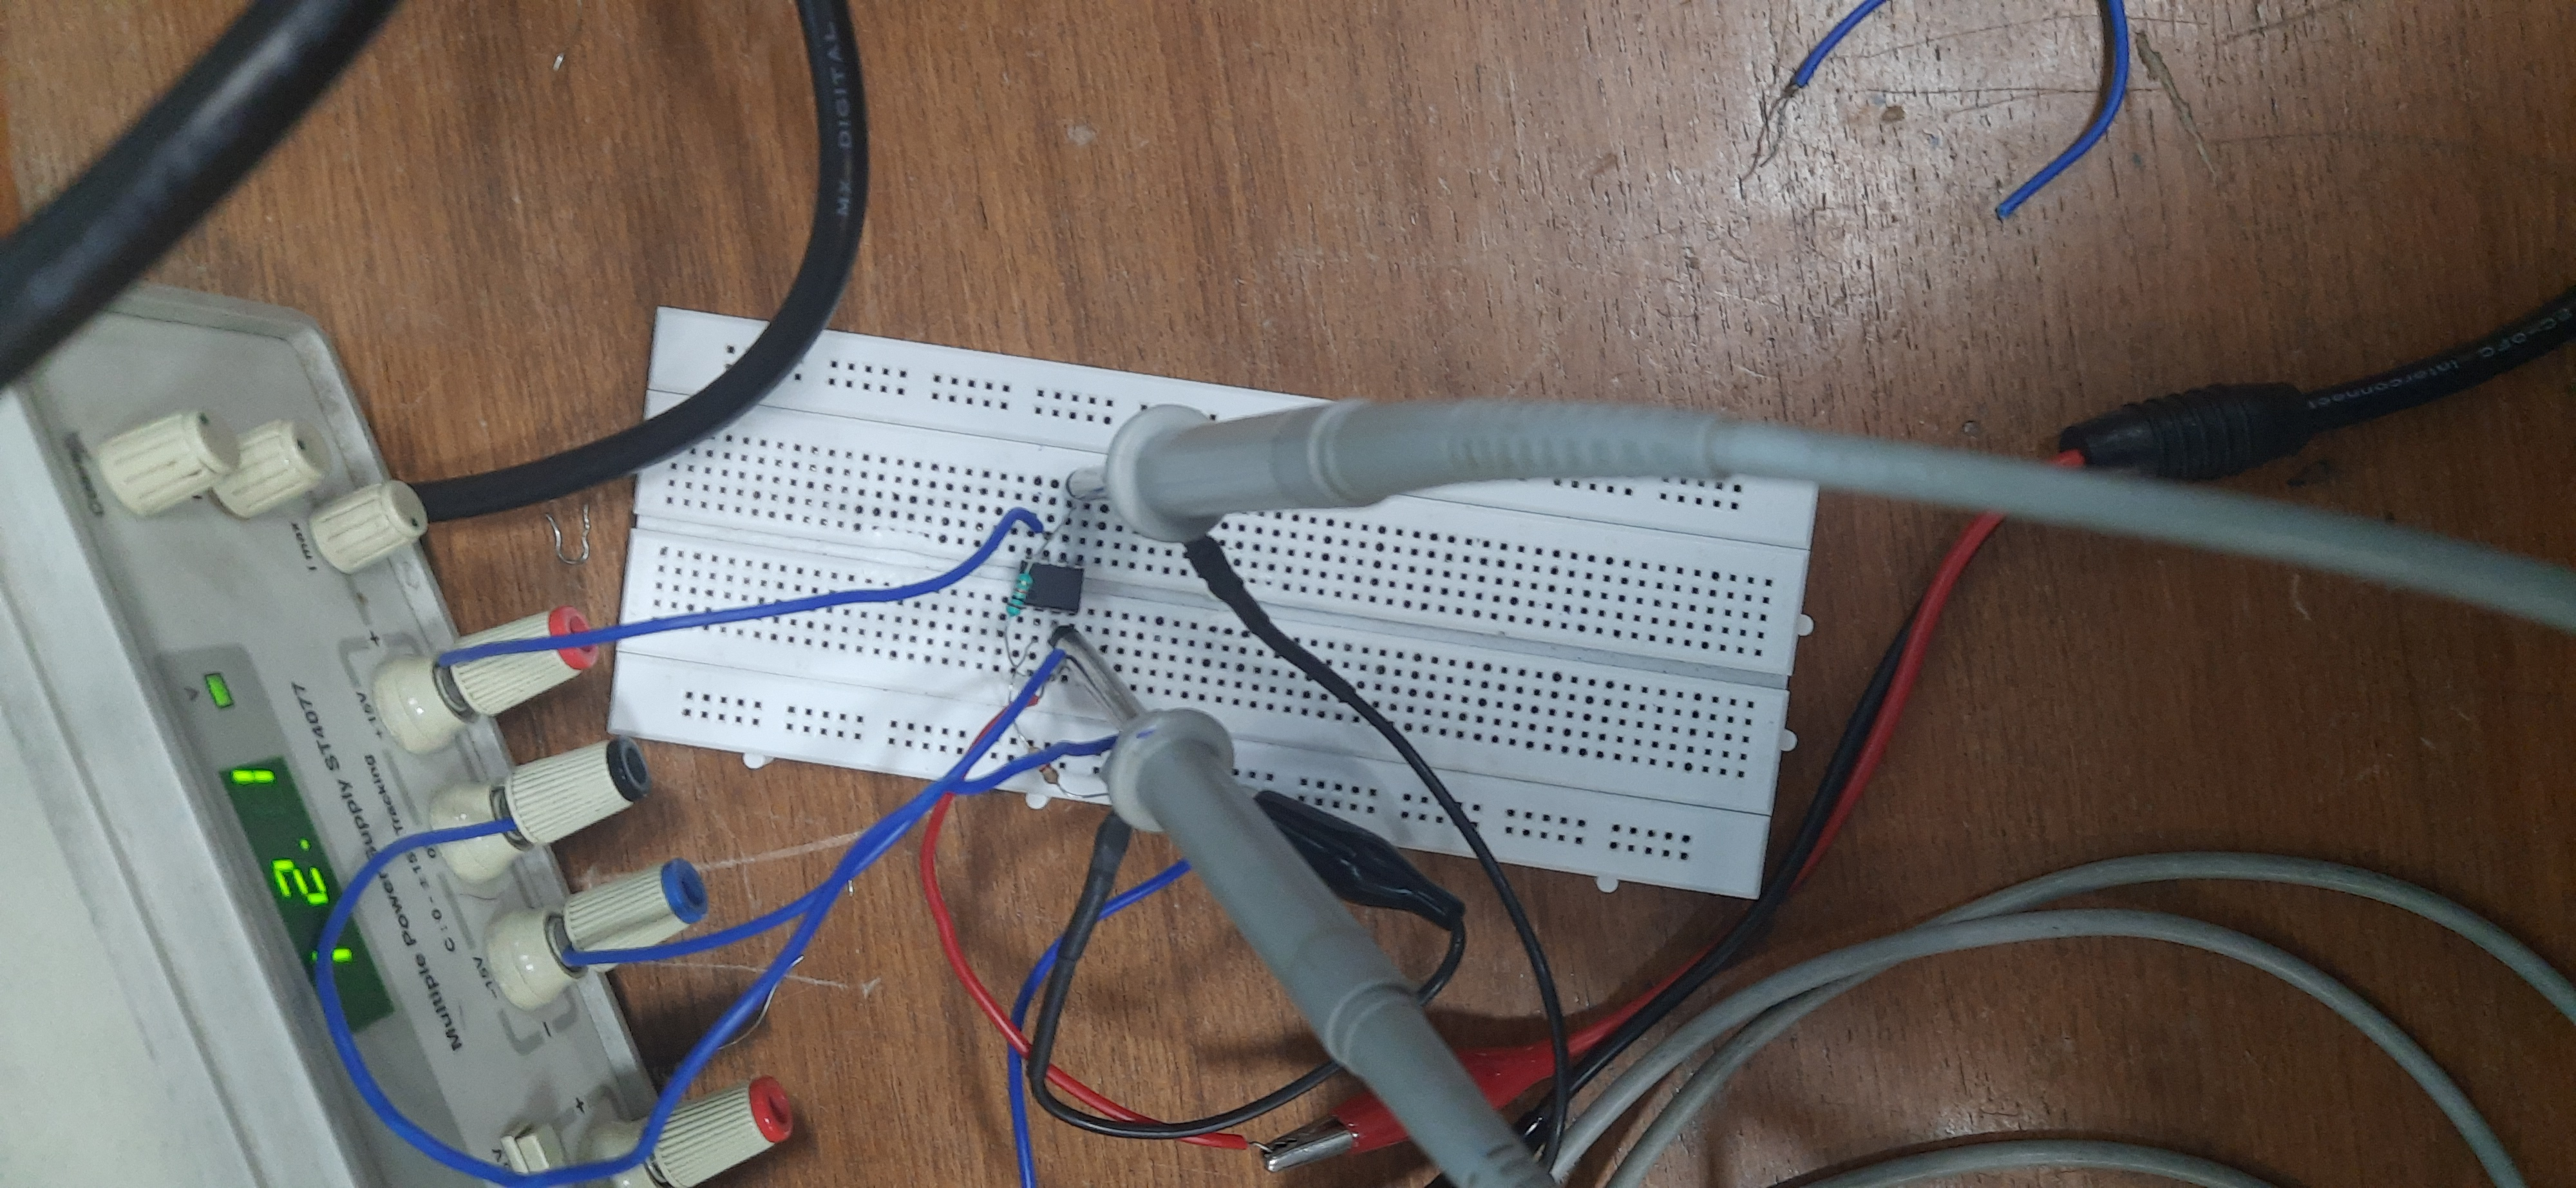
\includegraphics[width=0.9\columnwidth, height=150px]{20220517_163025.jpg}} \\ \vspace{5px}
Circuit with $R_{1}=1k\Omega$ and $R_{2}=10k\Omega$\\
\end{center}

\newpage
\subsection{Images of DSO}
\begin{multicols}{2}
\begin{center}
\fcolorbox{black}{white}{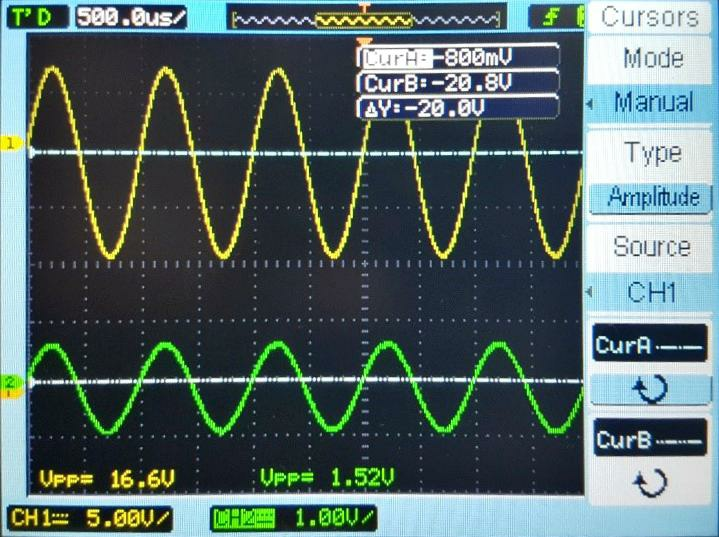
\includegraphics[width=0.9\columnwidth, height=110px]{WhatsApp Image 2022-05-31 at 9.48.30 PM (1).jpeg}} \\ \vspace{5px} 
F=1kHz \ $R_f=10k\Omega$ \\

\columnbreak

\fcolorbox{black}{white}{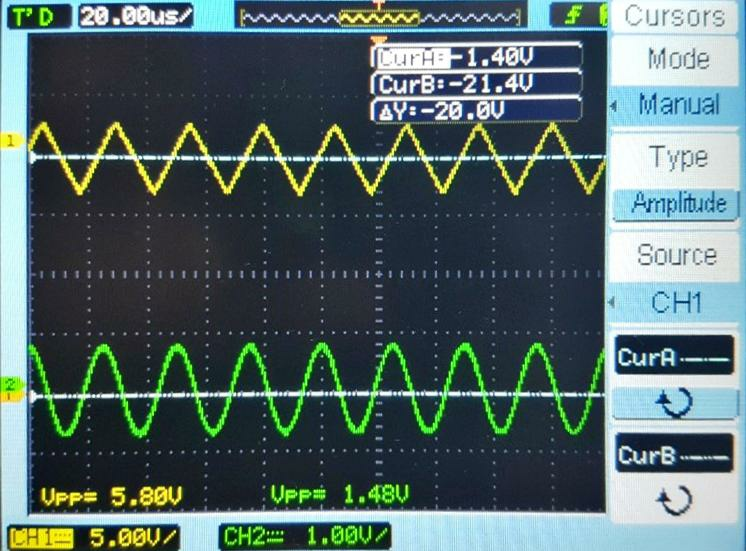
\includegraphics[width=0.9\columnwidth, height=110px]{WhatsApp Image 2022-05-31 at 9.48.30 PM (3).jpeg}} \\ \vspace{5px}
F=40kHz \ $R_f=10k\Omega$
\end{center}
\end{multicols}
\begin{multicols}{2}
\begin{center}
\fcolorbox{black}{white}{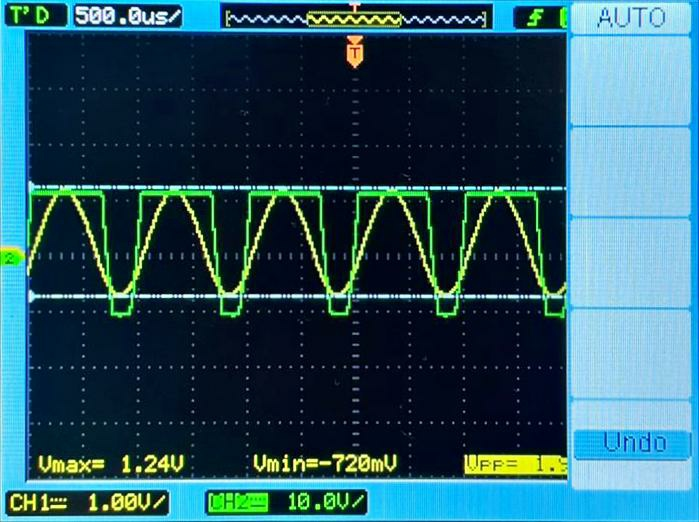
\includegraphics[width=0.9\columnwidth,  height=110px]{WhatsApp Image 2022-05-31 at 9.48.30 PM.jpeg}} \\ \vspace{5px}
F=1kHz \ $R_f=47k\Omega$ \\

\columnbreak

\fcolorbox{black}{white}{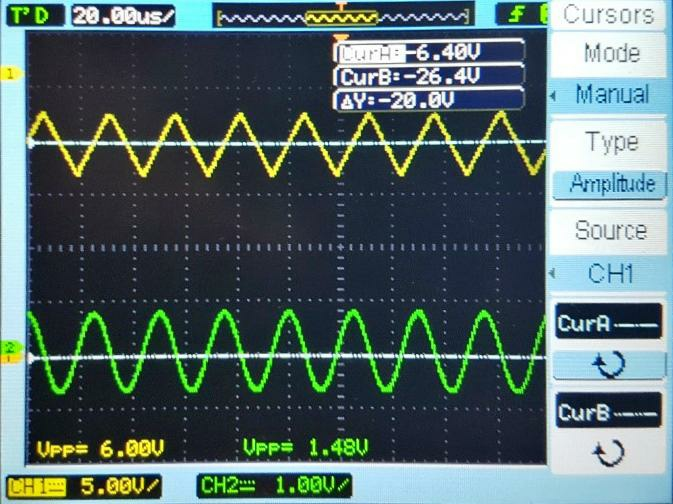
\includegraphics[width=0.9\columnwidth, height=110px]{WhatsApp Image 2022-05-31 at 9.48.30 PM (2).jpeg}} \\ \vspace{5px}
F=40kHz \ $R_f=47k\Omega$
\end{center}
\end{multicols}

\subsection{Observation}
\begin{center}
\begin{tabular}{| c | c | c |} 
 \hline
    \ & \ & \ \\
    Frequency and Resistance & $Input_{PP}$ & $Output_{PP}$ \\ [1em]
    \hline
    \ & \ & \ \\
    F=1kHz \ $R_f=10k\Omega$  & 1.5V & 15.5V \\
    F=40kHz \ $R_f=10k\Omega$  & 1.5V & 5.8V \\
    F=1kHz \ $R_f=47k\Omega$  & 1.5V & 22.4V \\
    F=40kHz \ $R_f=47k\Omega$  & 1.5V & 6.2V \\
    \ & \ & \ \\
 \hline
\end{tabular}
\end{center}

\subsection{Conclusion}
We see that the current is in almost the same phase in lower frequencies and slightly different at higher frequencies. Also, the voltage gain values are almost correct for low frequencies( except where the output voltage exceeds the 24V supplied voltage.


\newpage
\vspace{10px}
\section{Sources of Error}
\begin{itemize}
\item Scale of DSO not appropriate for measurements
\item Loose Connections
\item Resistance of wires not taken into account, and also giving rise to inconsistency due to increase in resistance due to heating
\item Change in the connections while circuit is closed.

\end{itemize}

\vspace{5px}

\section{Precautions}

\begin{itemize}
\item Make the connections neat and tight
\item Don’t leave the switch on for long continuous periods of time.
\item Wear proper shoes and use insulated tools
\end{itemize}

\vspace{5px}

\section{Concluding Remarks}
In the first part of the experiment, we observe that the voltage across the resistance was quite different from that of the input voltage and had different phase. However, the voltage from the voltage follower was almost the same with the same phase. \\

In the second part of the experiment, we saw that the output voltage across an inverting amplifier. We also saw that the value of output voltage is exactly 10 times the input voltage for $R_f = 10k\Omega$, which adheres to the formula. In the higher frequency shift we see higher deviations from expected results. This is owing to the reason that the breakpoint of the op-amp is exceeded at 40 kHz. At this rate the slew rate becomes comparable to the signal frequency. Thus, resulting into erratic behavior. \\

In the third part of the experiment we saw the output waveform from a non-inverting op-amp. The maximum limit exceeded the supplied voltage in the $47 k\Omega$ resistor case. Also the same triangular waves were observed in higher frequencies due to breakpoint. \\

Thus, in the above experiment, we studied the characteristics and some applications of the operational amplifier- as a voltage follower, as an inverting amplifier and as a non-inverting amplifier. We studied what gain is, and experimentally verified the gain for these different configurations of the operational amplifier.
\end{document}
